%use the KomaScript styling on A4 paper
\documentclass[a4paper]{scrreprt}
%package for citing in Harvard style
\usepackage{natbib}
\bibliographystyle{agsm}
\usepackage[T1]{fontenc}
\usepackage[utf8]{inputenc}
\usepackage{graphicx}
\graphicspath{{"./figs"}}

\begin{document}

\begin{titlepage}
\centering
{\large\textsc{Bachelor thesis}\par}
\vspace{8\baselineskip}
{\Huge The right-wing populism of the AfD party and its regional differences\par}
\vspace{2\baselineskip}
{\Large A quantitative analysis on populist antagonisms within the programmatic discourse\par}
\vspace{5\baselineskip}
{\large\textsc{submitted by\\[.5em]Dipl.-Math. Paul Keydel}}
\vfill
{\em Freie Universität Berlin, April 2024}
\end{titlepage}

\tableofcontents

%%%%%
% 1 %
%%%%%
\chapter{Introduction}
The aim of this thesis is to bla bla
%%%%%
% 2 %
%%%%%
\chapter{Populism as ideology of the democracy}
\section{What is an ideology?}
\section{Populism: the bridge between \guilsinglright the people\guilsinglleft\ and \guilsinglright the politics\guilsinglleft}
\section{The role of antagonisms}
%%%%%
% 3 %
%%%%%
\chapter{The AfD party and its right-wing populism}
\section{Usage of right-wing antagonisms and recent developments in federal states}
\section{Towards an analysis of the programmatic discourse}
%%%%%
% 4 %
%%%%%
\chapter{An analysis of antagonisms within AfD manifestos}
\section{Methodological considerations: A dictionary-based approach}
\begin{figure}
    \centering
    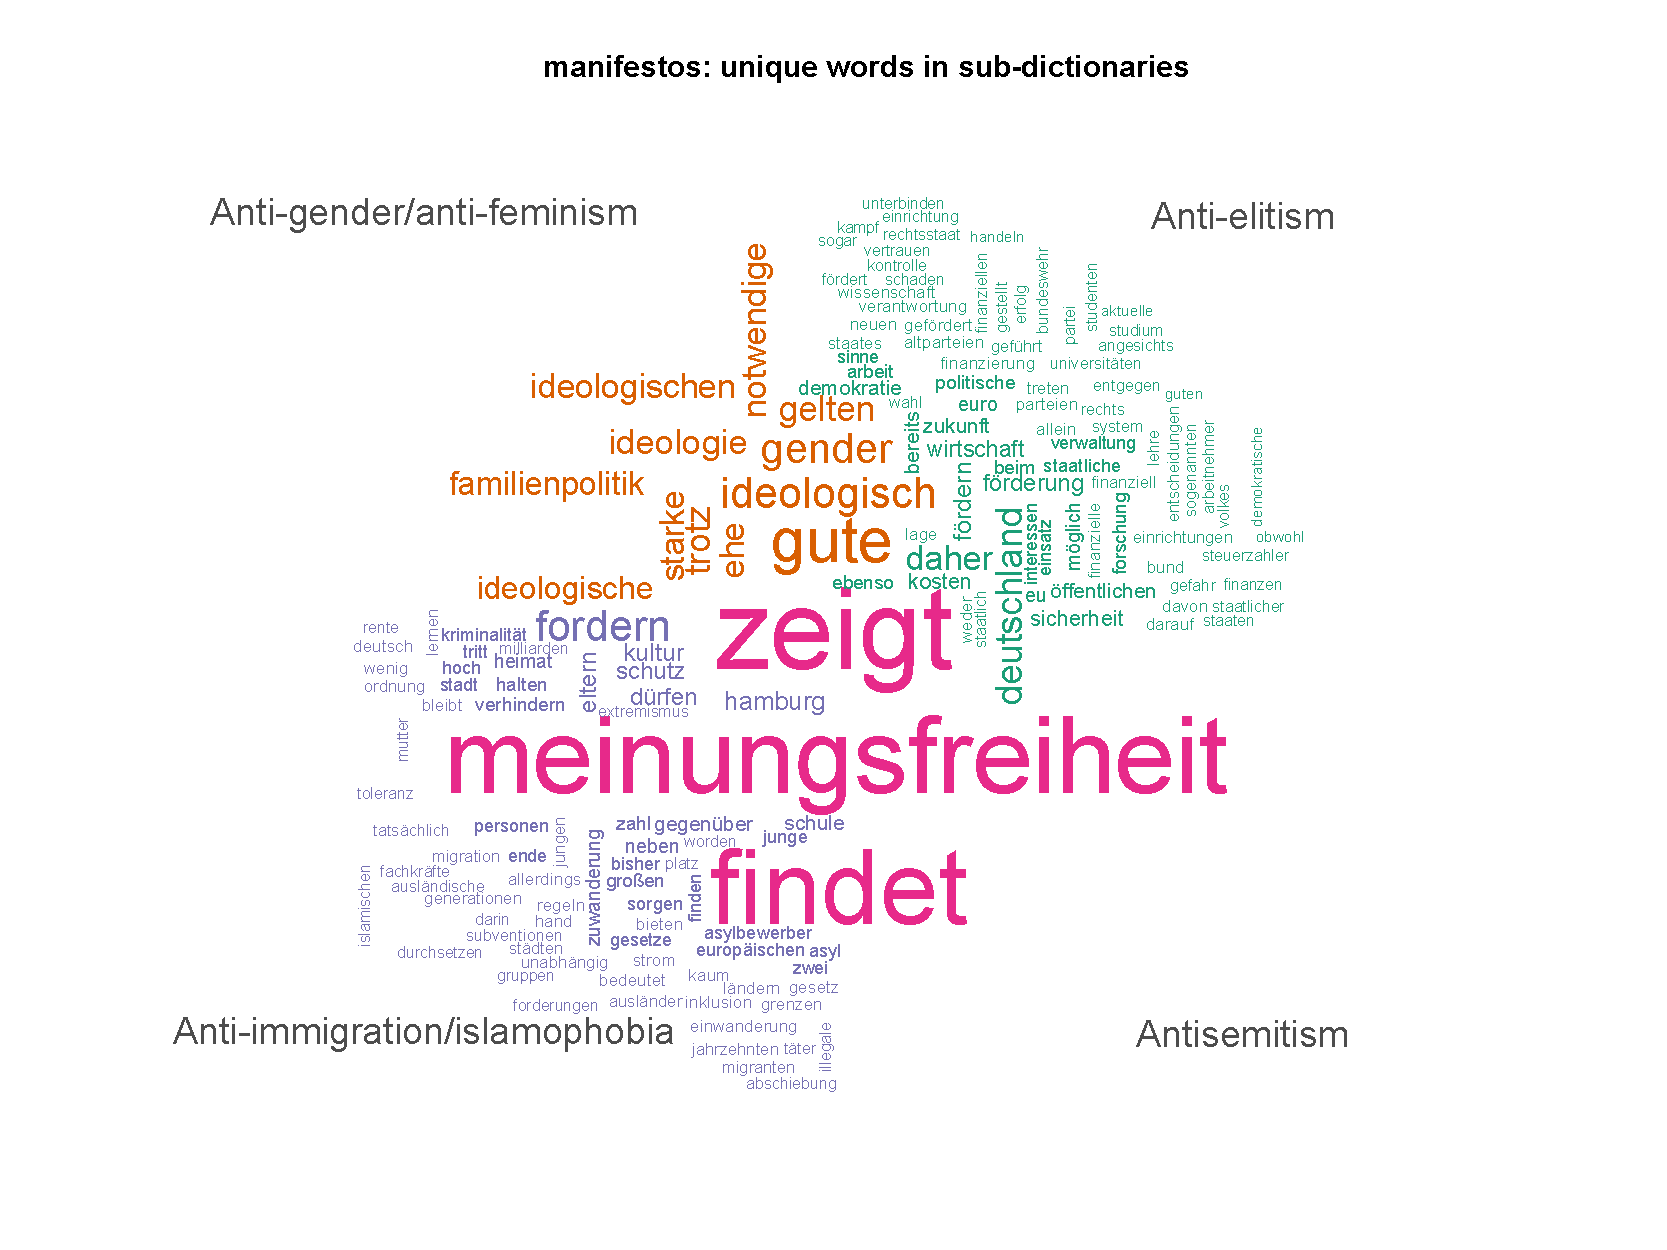
\includegraphics[width=0.9\textwidth]{manifestos_unique_words_subdicts.pdf}
    \caption{a nice plot}
\end{figure}
\section{Results for the last two state elections}
\begin{figure}
    \centering
    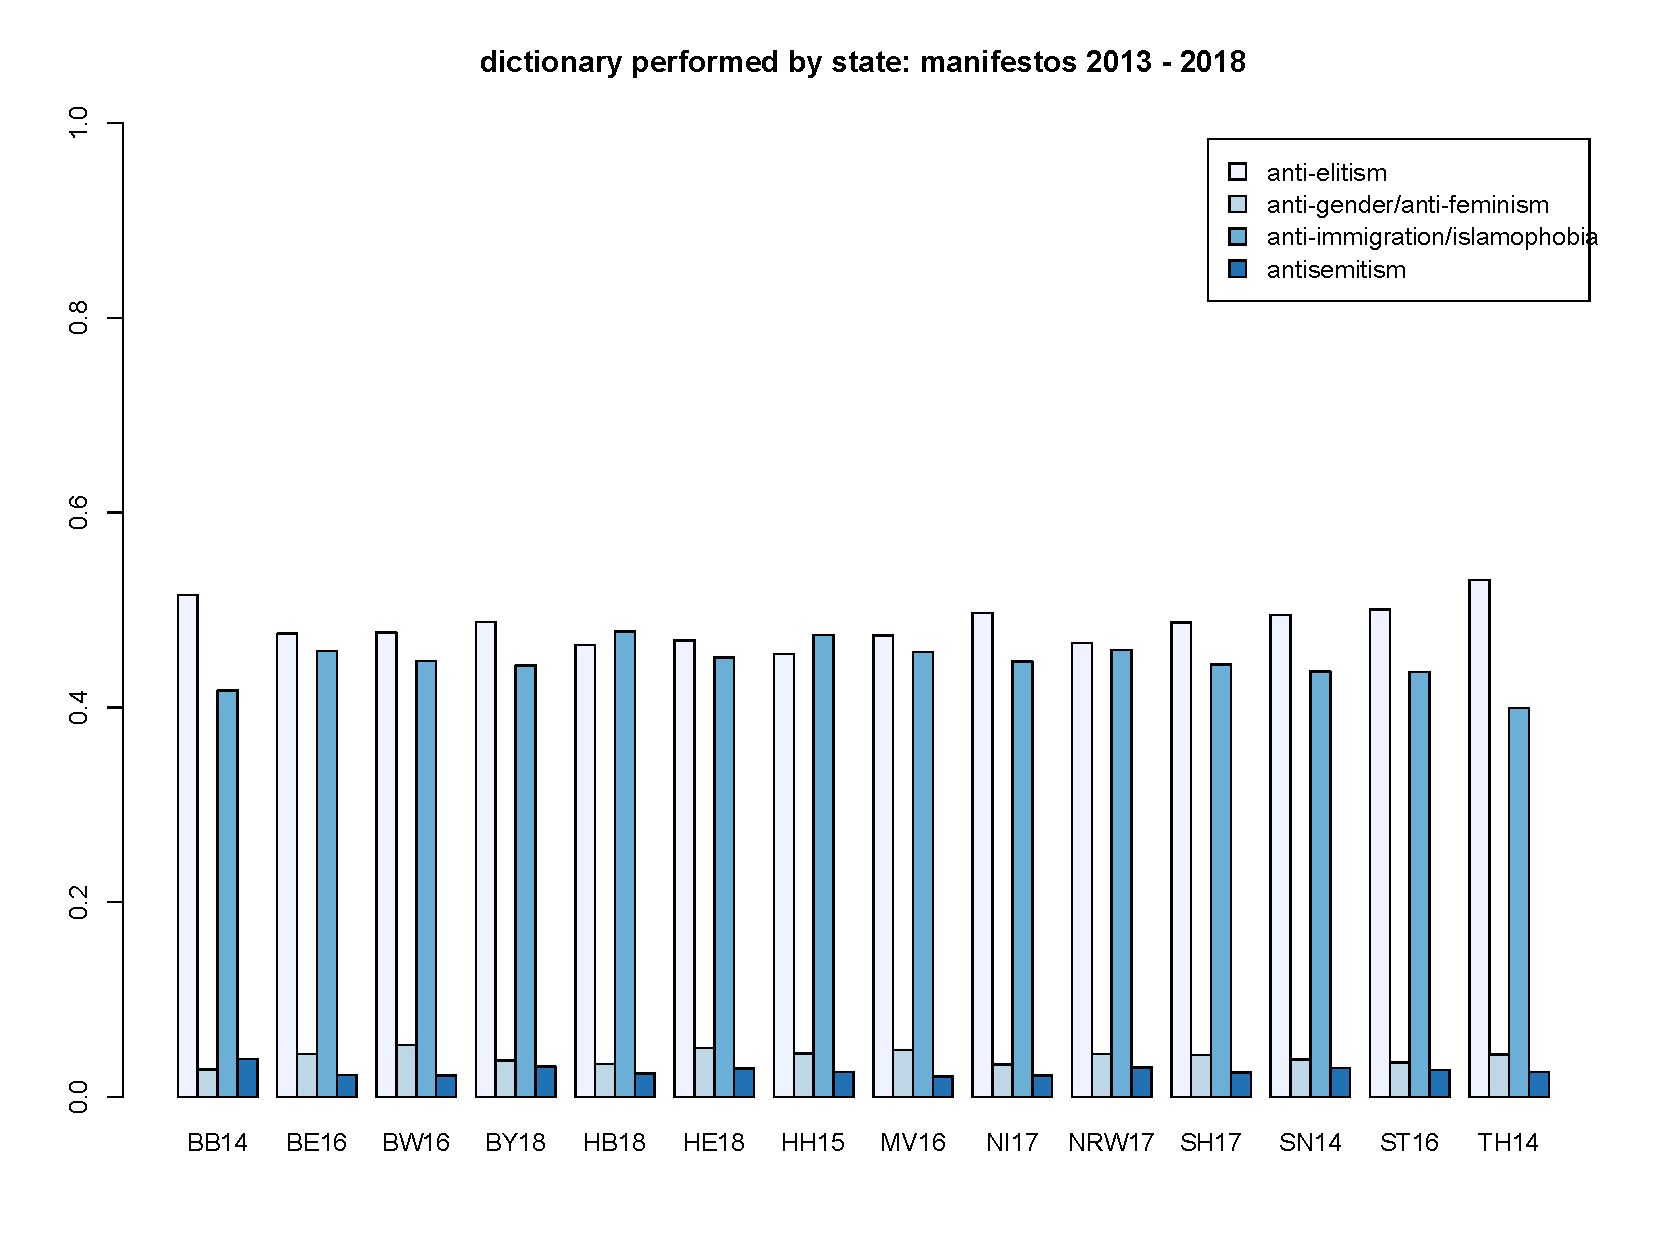
\includegraphics[width=\textwidth]{manifestos_dict_states_2013.pdf}
    \caption{a nice plot}
\end{figure}
\begin{figure}
    \centering
    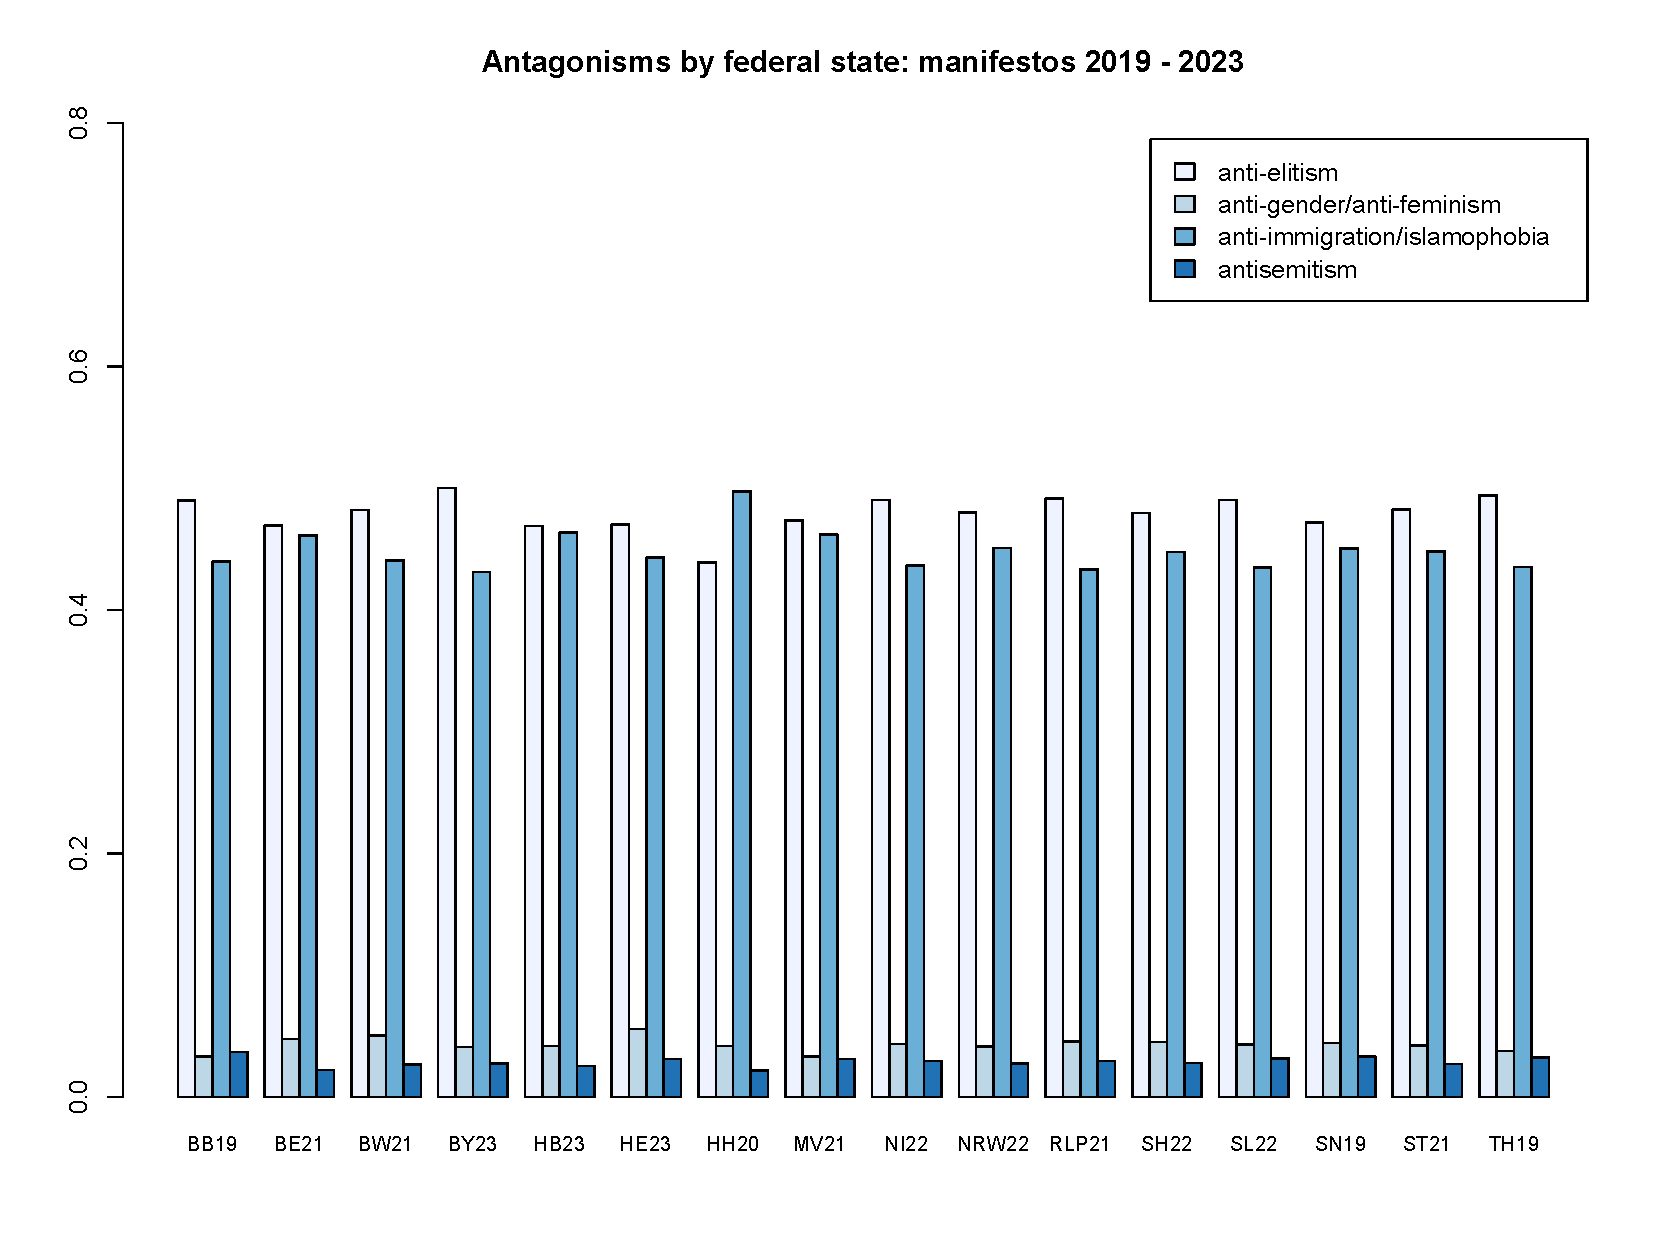
\includegraphics[width=\textwidth]{manifestos_dict_states_2018.pdf}
    \caption{a nice plot}
\end{figure}
\section{Temporal changes between East and West Germany}
\begin{figure}
    \centering
    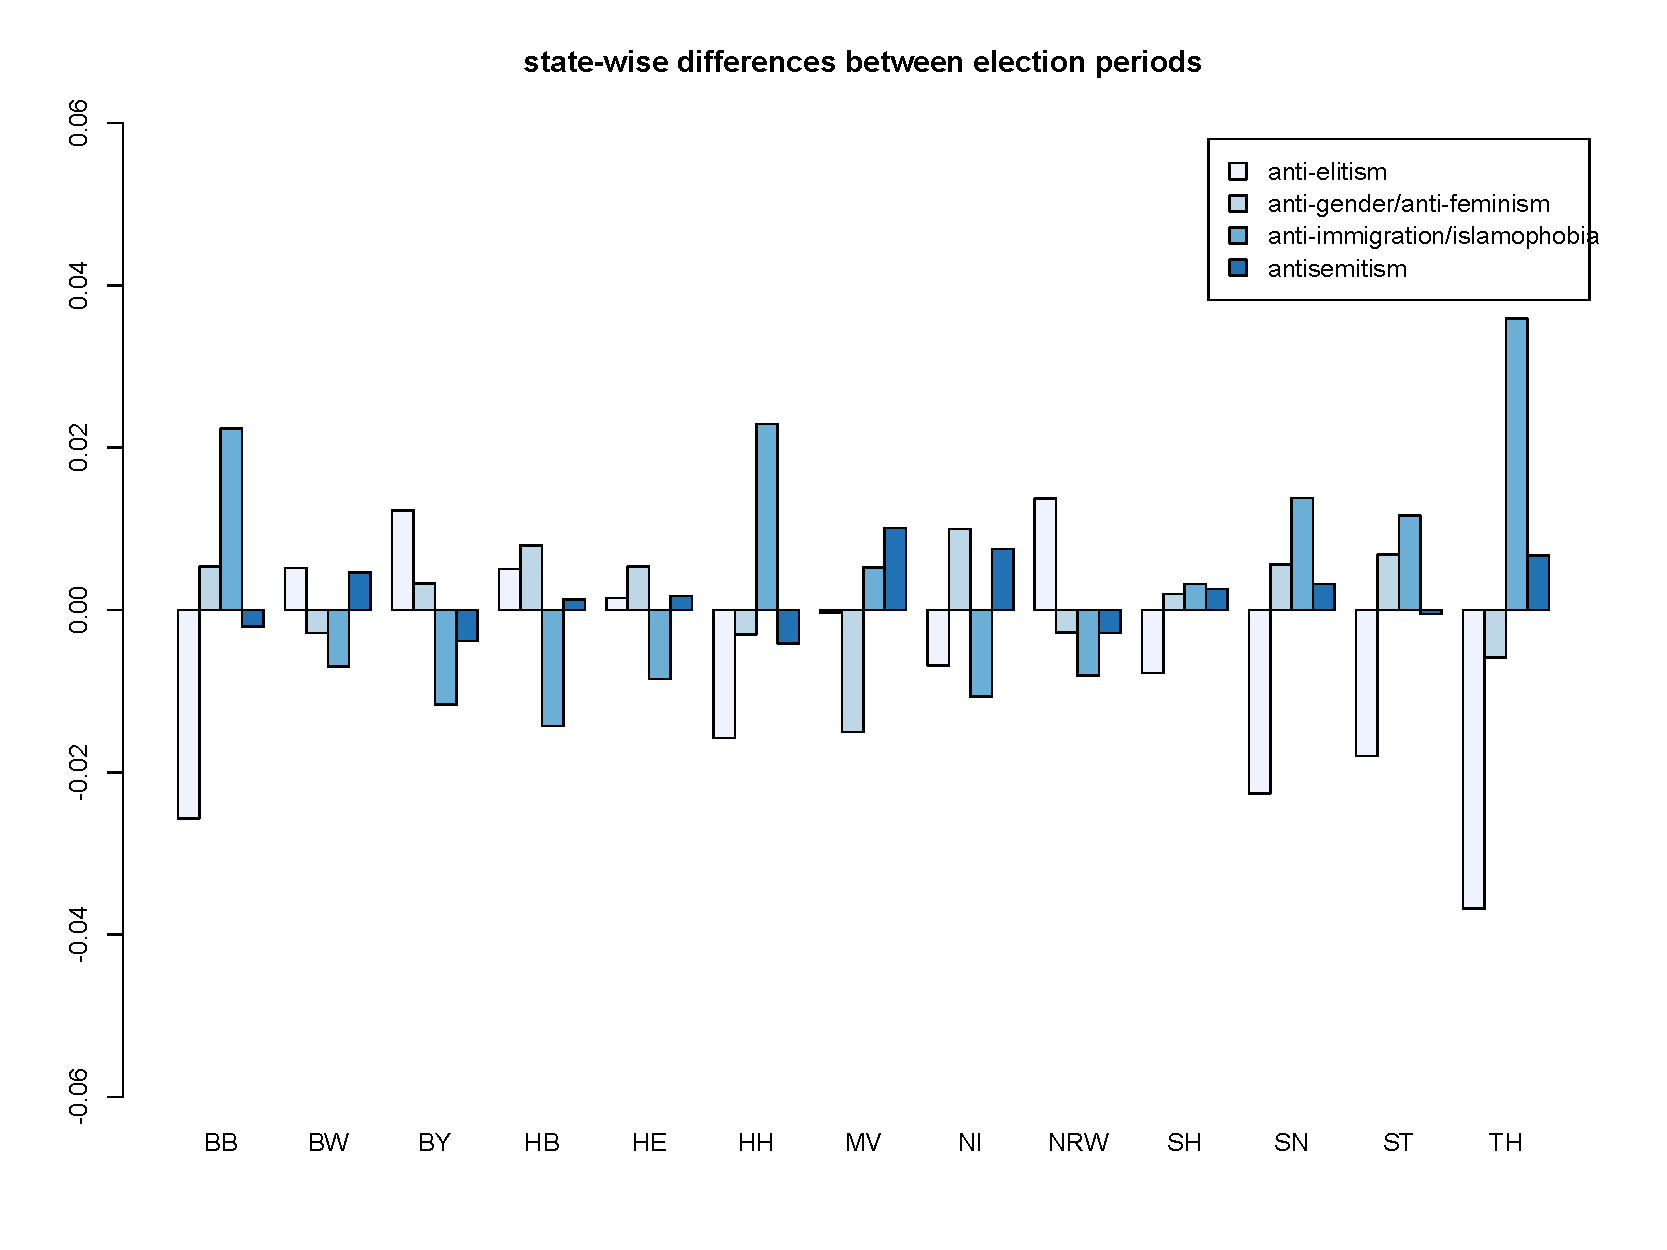
\includegraphics[width=\textwidth]{manifestos_dict_states_diffs.pdf}
    \caption{a nice plot}
\end{figure}
\begin{figure}
    \centering
    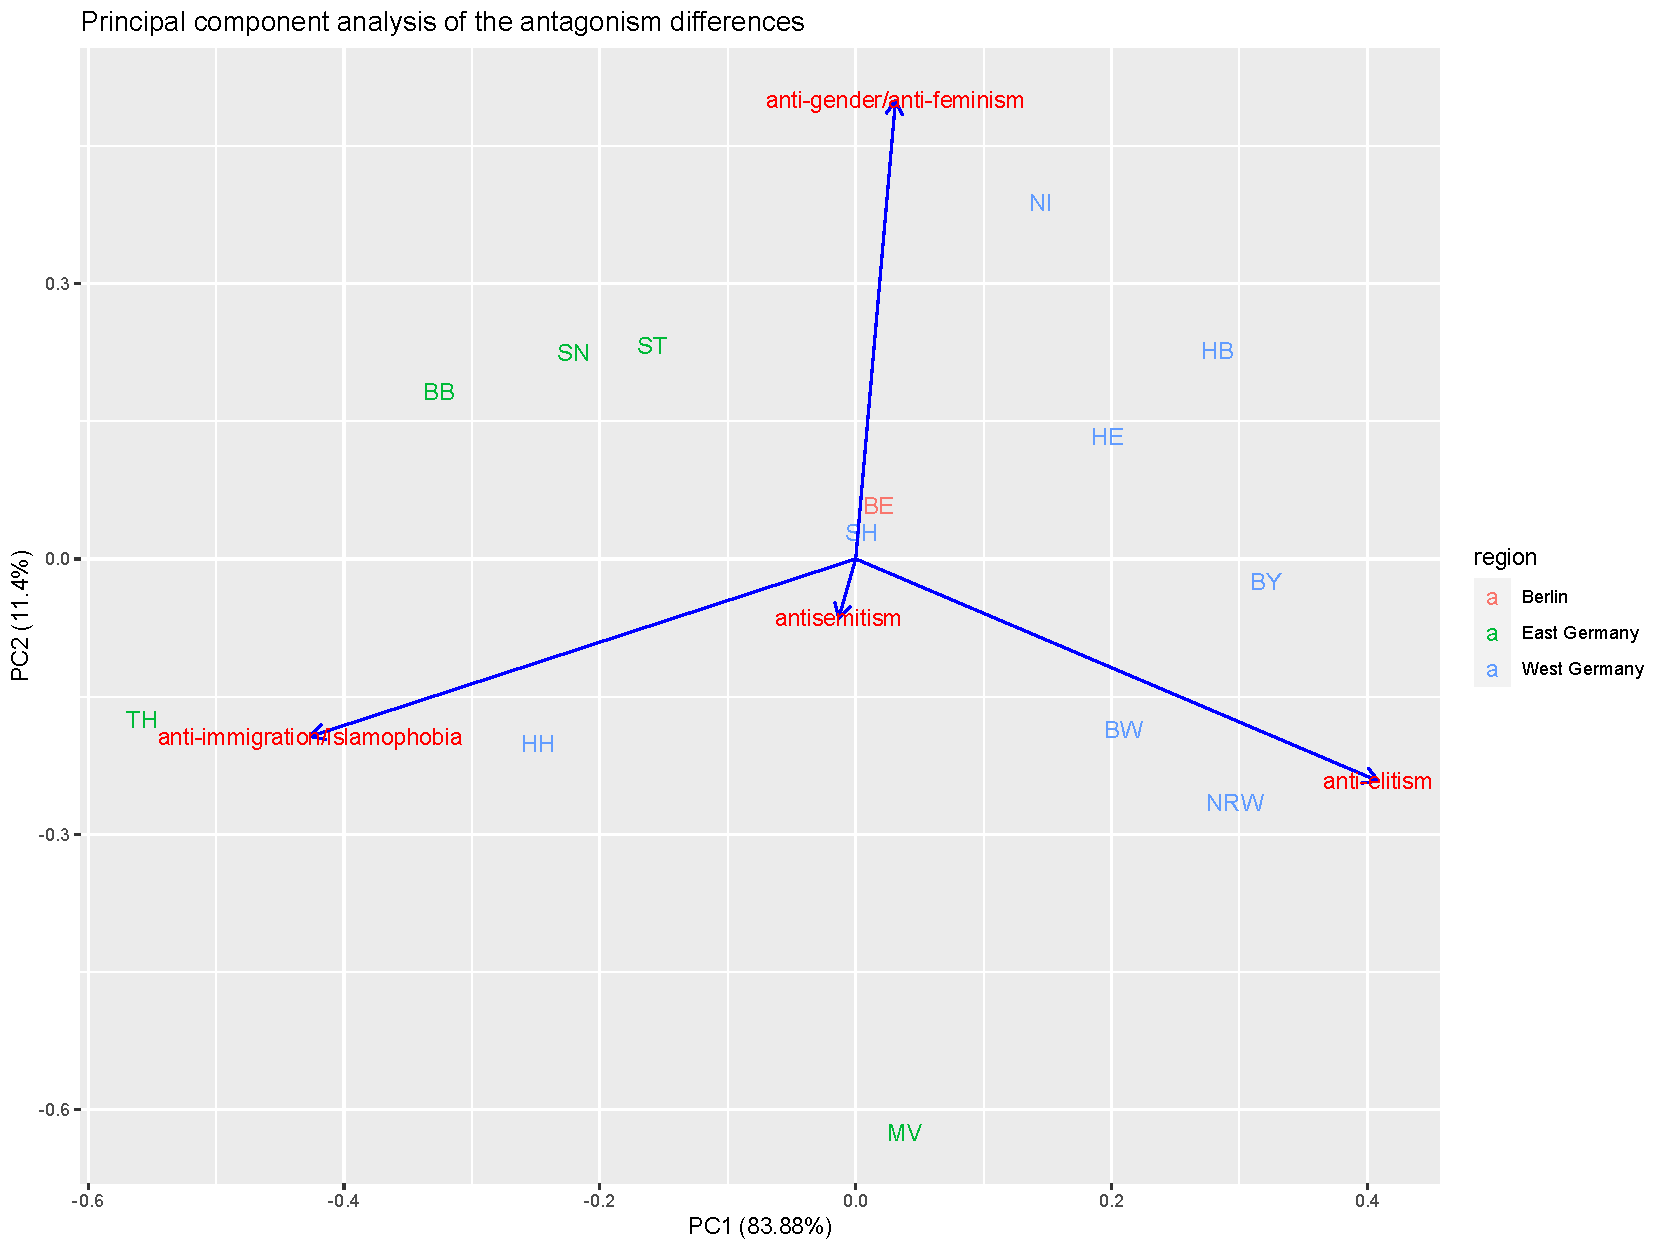
\includegraphics[width=\textwidth]{manifestos_diffs_pca.pdf}
    \caption{a nice plot}
\end{figure}
\begin{figure}
    \centering
    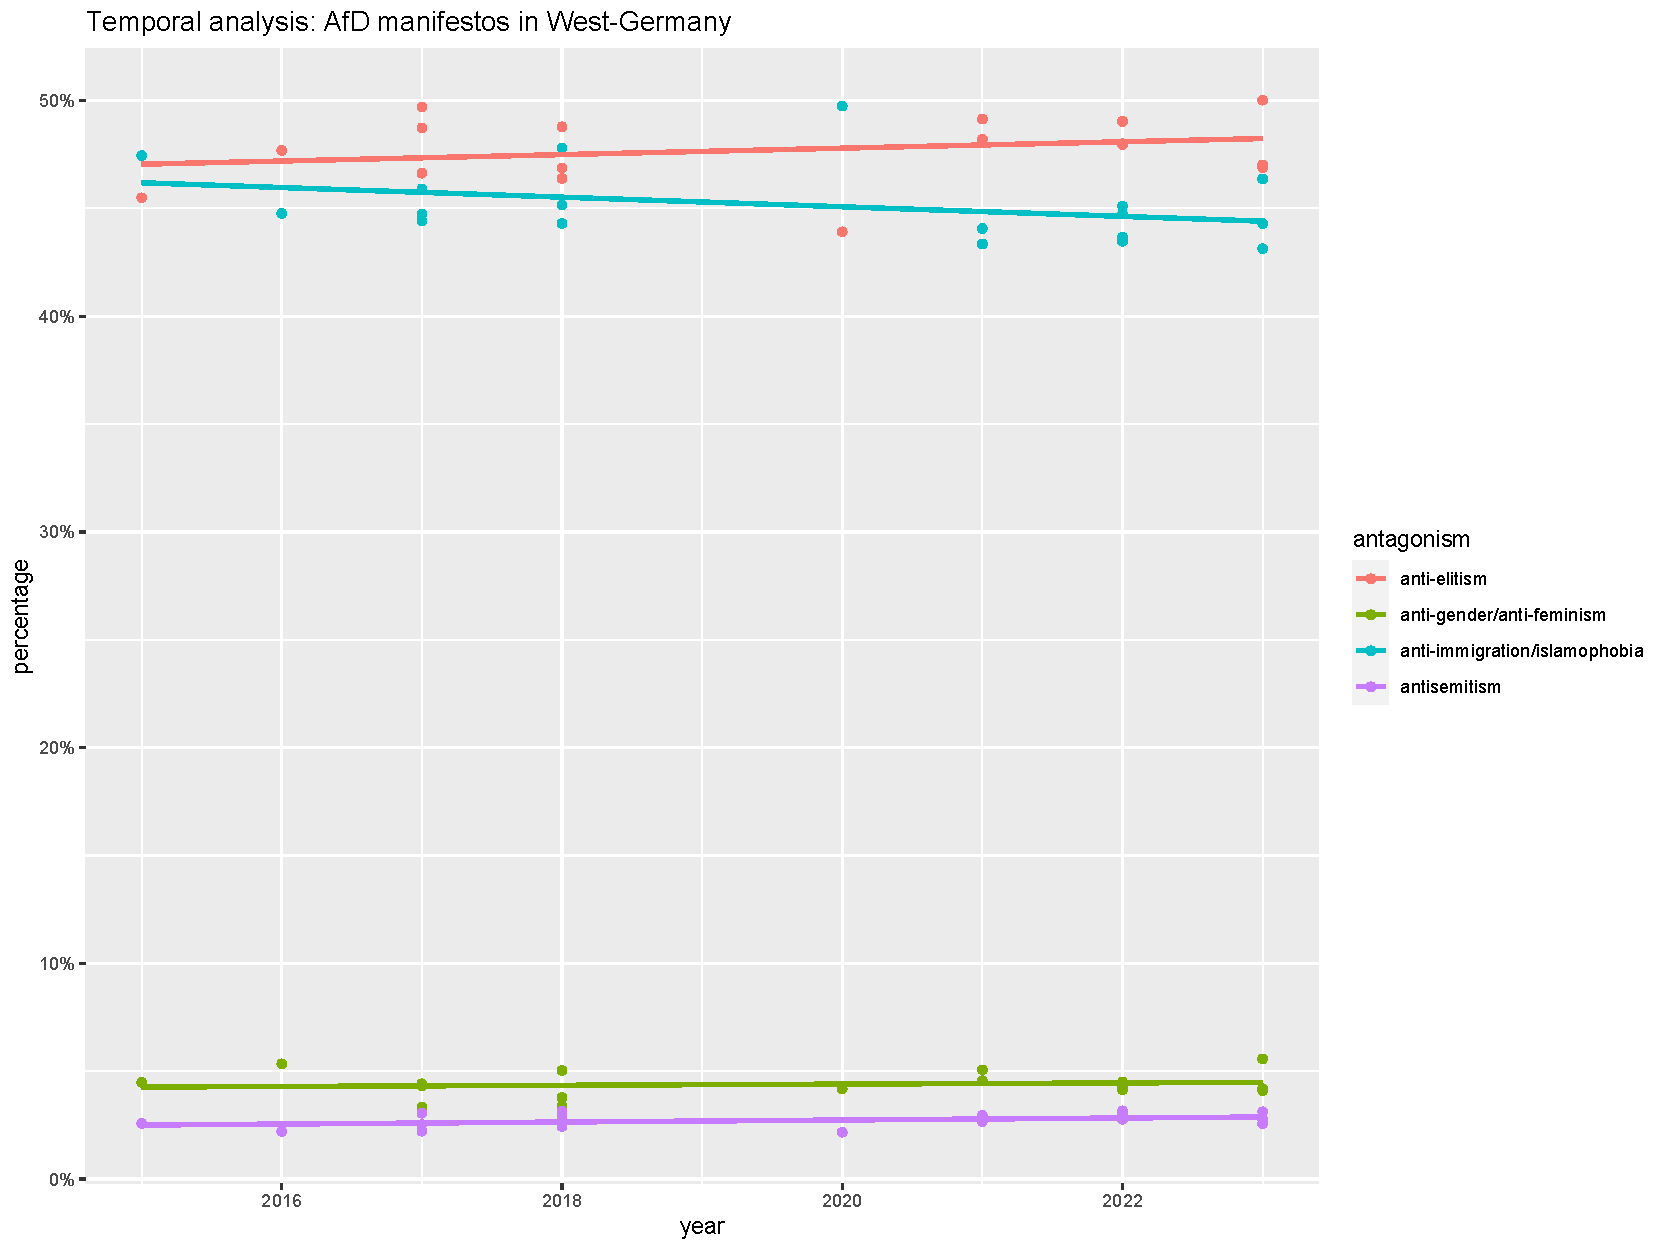
\includegraphics[width=\textwidth]{manifestos_temporal_regression_west.pdf}
    \caption{a nice plot}
\end{figure}
\begin{figure}
    \centering
    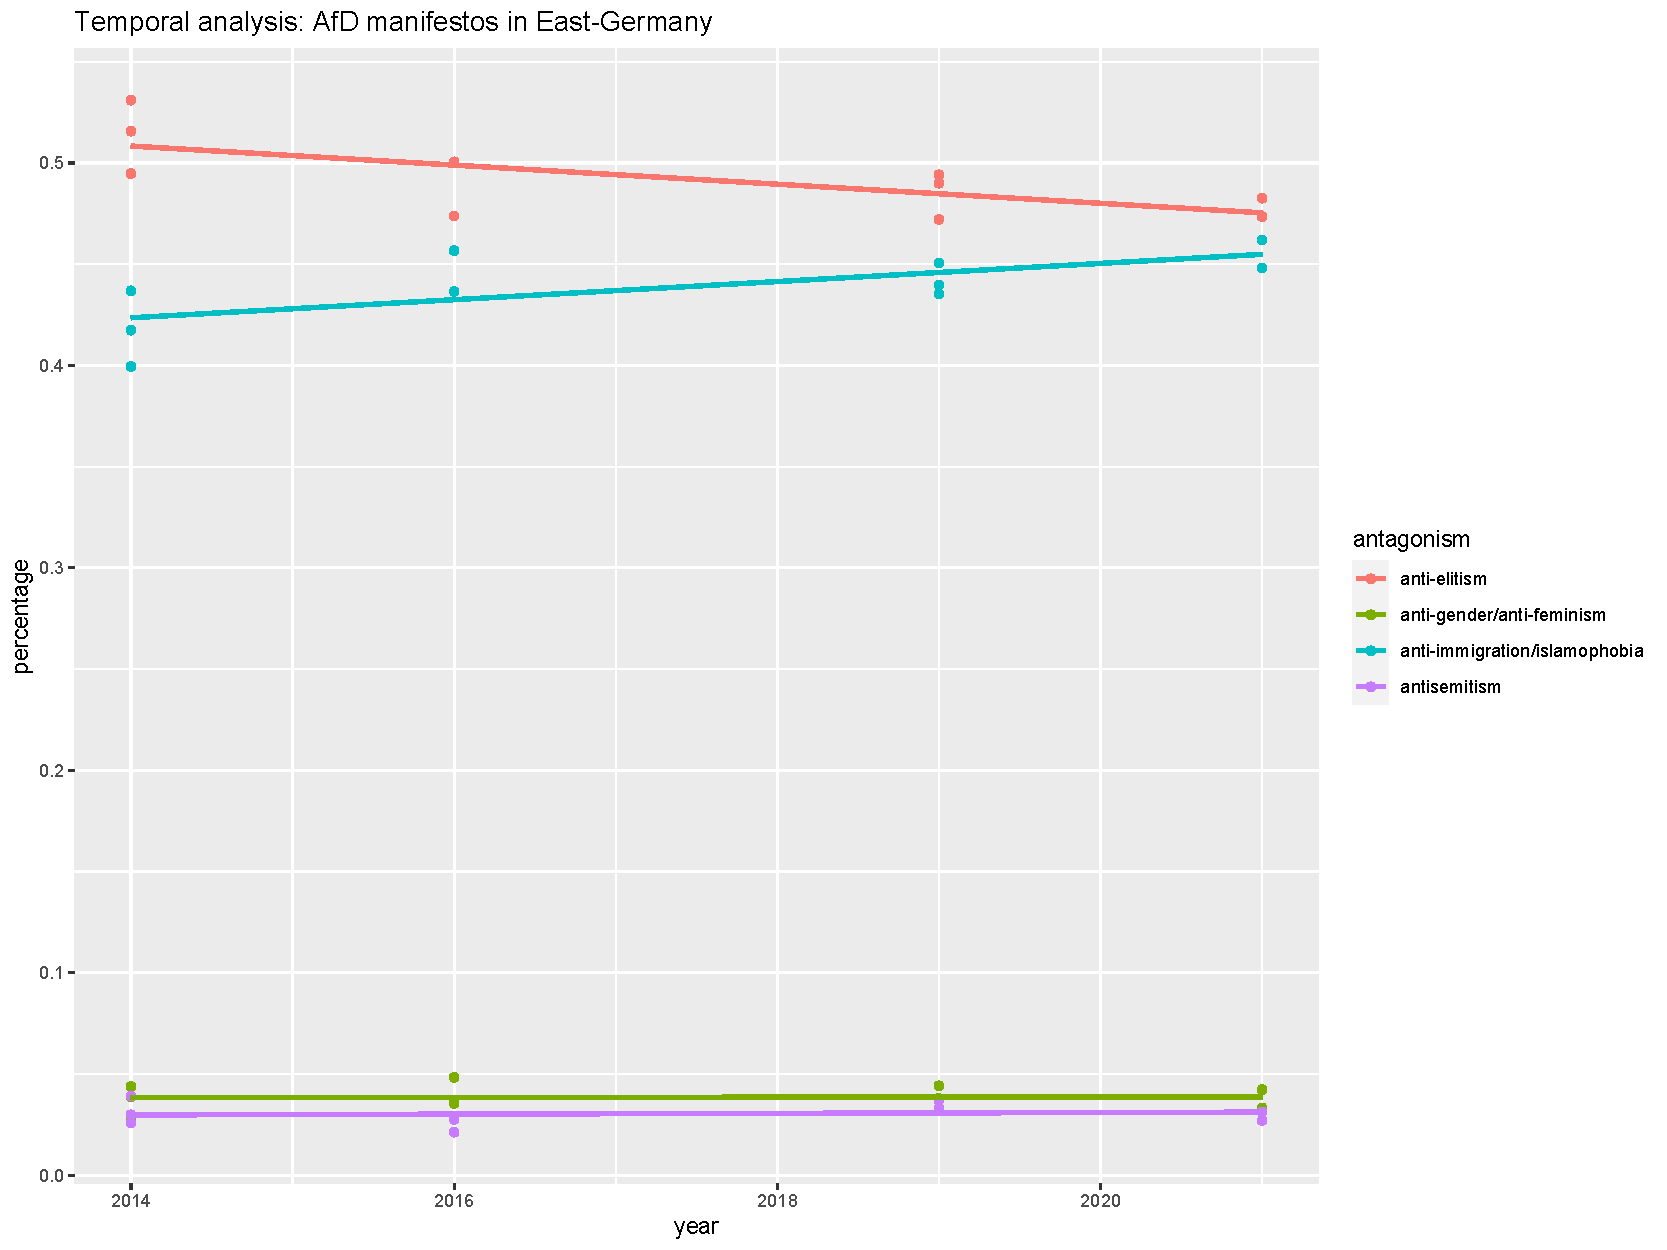
\includegraphics[width=\textwidth]{manifestos_temporal_regression_east.pdf}
    \caption{a nice plot}
\end{figure}
%%%%%
% 5 %
%%%%%
\chapter{Evaluation of the findings and validation}
\begin{figure}
    \centering
    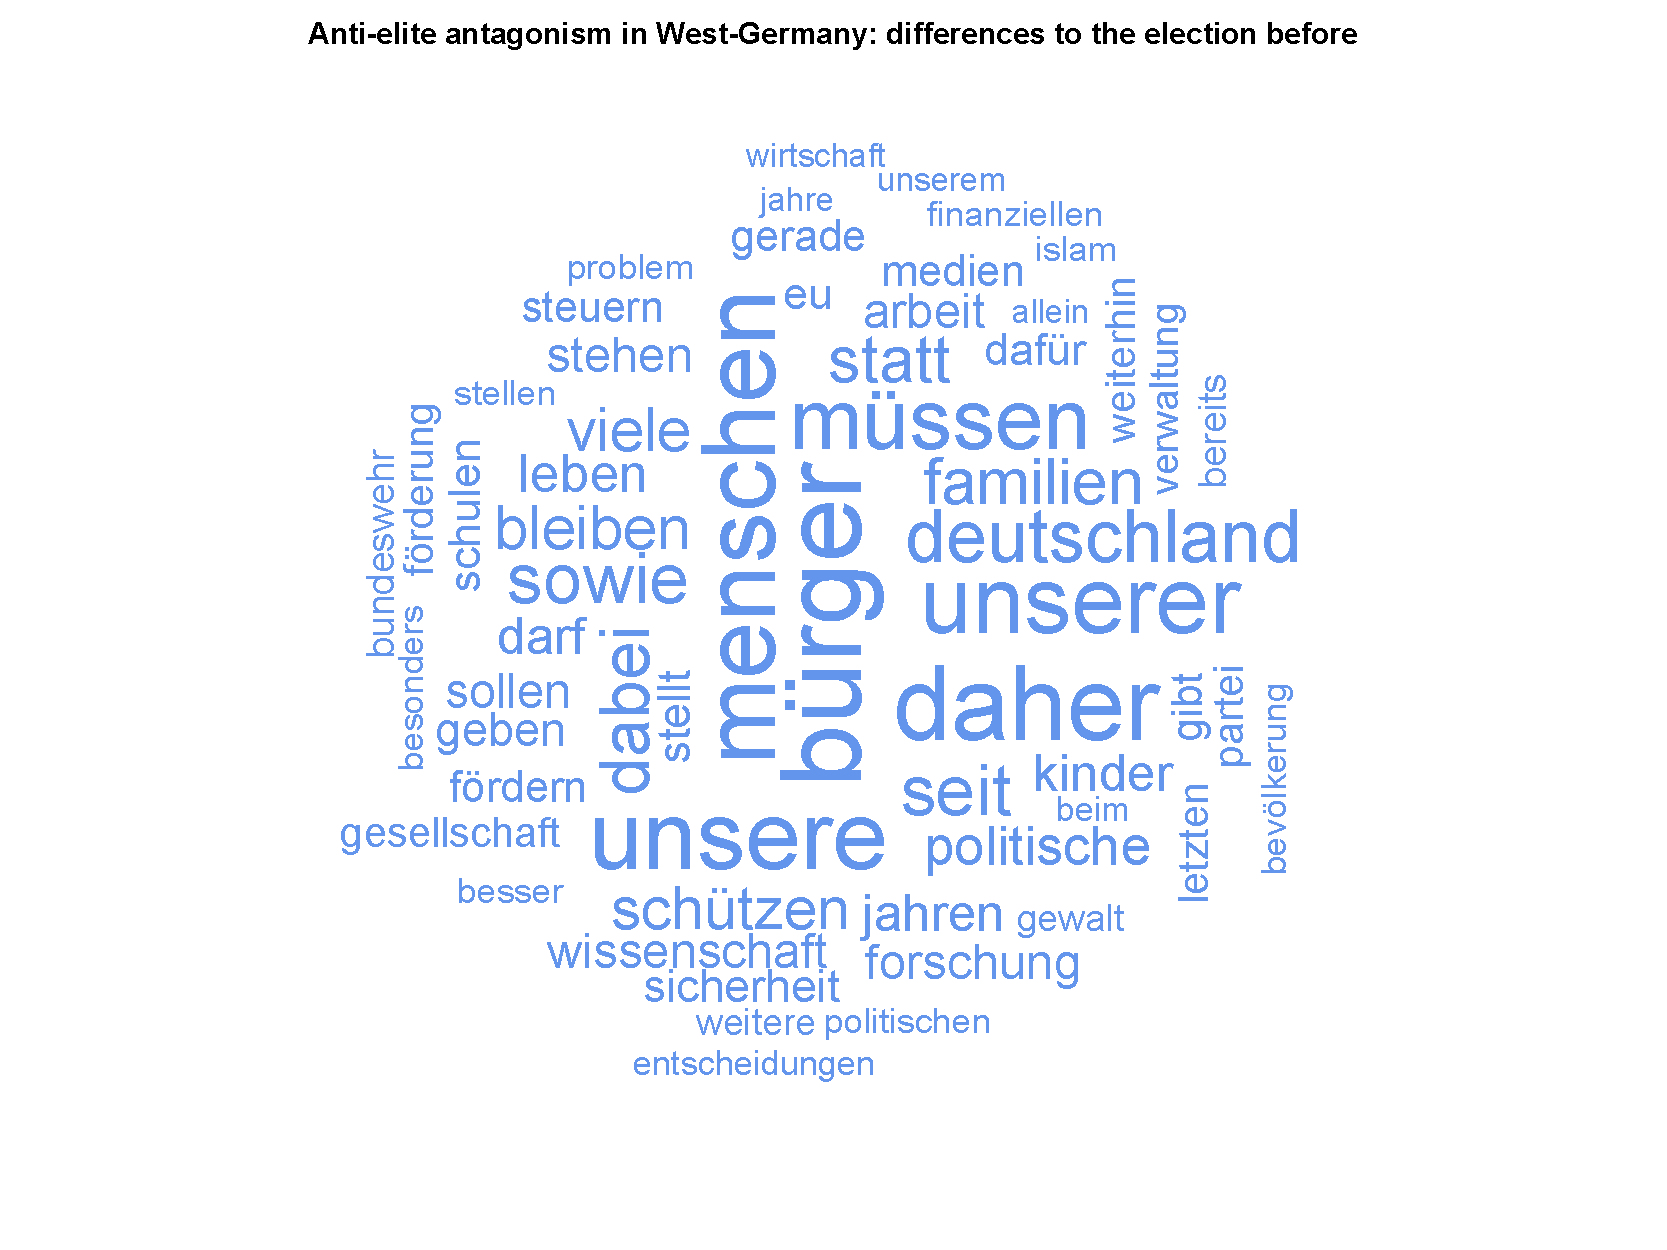
\includegraphics[width=0.9\textwidth]{manifestos_wordcloud_diffs_west.pdf}
    \caption{a nice plot}
\end{figure}
\begin{figure}
    \centering
    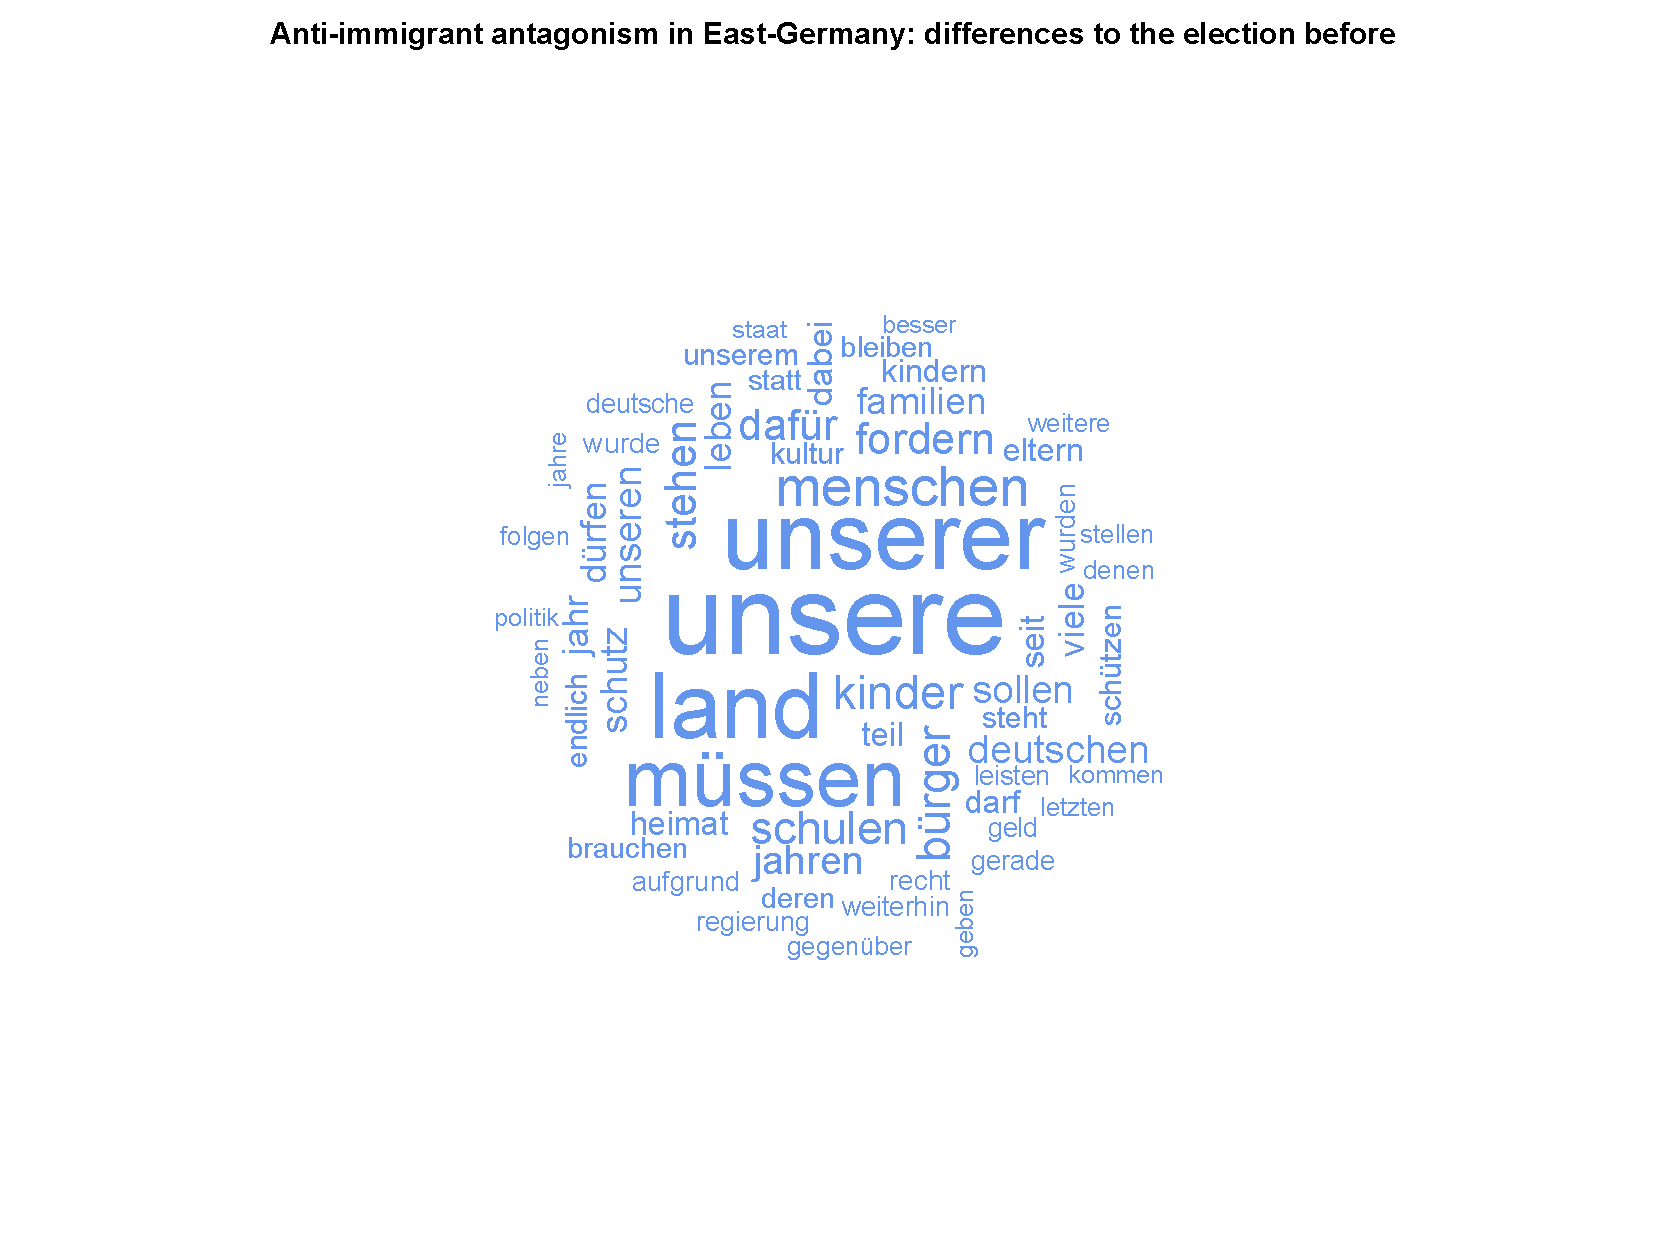
\includegraphics[width=0.9\textwidth]{manifestos_wordcloud_diffs_east.pdf}
    \caption{a nice plot}
\end{figure}
%%%%%
% 6 %
%%%%%
\chapter{Conclusion and final comments}
Let's start citing \citep[p.~22]{canovan:2002}

\bibliography{refs}

\end{document}